If you have a research bent, by this point, you may be asking yourself
questions like these: \emph{How can we understand peer learning better?}
\emph{How can we do research ``the peeragogical way''?} \emph{How do we
combine research and peer learning?}You may also be asking more
technical methodological and instrumentation-level questions: \emph{Do
we have a good way to measure learning?} \emph{Which activities and
interventions have the biggest payoff?} This chapter summarizes
socio-technical research I did on PlanetMath, using the pattern catalog,
as part of my work for my PhD. In the course of the study, I developed 3
new patterns. The first point to make is that although this research was
informal, it is nevertheless (at least in my view) highly rigorous. This
is because the pattern catalog is a relatively stable, socially agreed
upon objct, though it is not fixed for all time. We can use it to help
identify ``known'' patterns, but we can also extend it, as needed, with
new patterns - assuming that we can make an argument to explain why the
new patterns are needed. The notion of pattern-finding as a process
related to, but distinct from abstraction is described by Richard
Gabriel, who emphasizes that the ``patterns and the social process for
applying them are designed to produce organic order through piecemeal
growth'' {[}1{]}, p. 31. We can use the rigorous-but-informal notion of
an expanding pattern catalog to help address the high-level questions
about peeragogical research mentioned above. The three new patterns I
present here are: Frontend and Backend, Spanning Set, and Minimum Viable
Project. These patterns are both an ``outcome'' of research in a real
peer learning context - and also a reflection on peeragogical research
methods. Like the other peeragogy patterns, they are tools you can use
in your own work. In particular, I hope this short essay will help you
use the peeragogy pattern catalog to constructively evaluate your own
peeragogy projects.

\subsection{Study design}

The study was based on interviews with users of a new software system
that we deployed on PlanetMath.org. In the interviews, we covered a wide
range issues, ranging from basic issues of usability all the way to
``deep'' issues about how people think about mathematics. In this
project, I was interested not only in how people collaborate to solve
mathematical problems, but how they think about ``system level'' issues.
The design I had in mind is depicted in the figures below. The key idea
is that patterns emerge as ``paths in the grass'', or ``desire lines''.
The idea that learning design has emergent features is not itself new
(see e.g. {[}2{]}): what's new here is a characterization of the key
patterns for \emph{doing} emergent design in a peer learning context.

\begin{figure}
\begin{center}
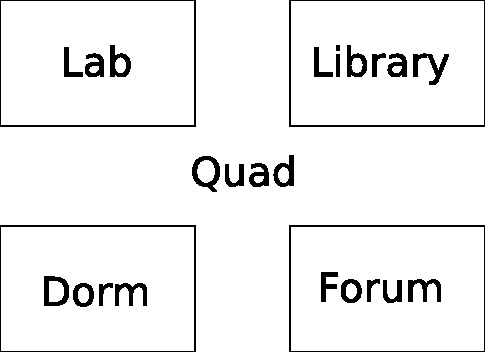
\includegraphics[width=.7\textwidth]{../pictures/PeeragogyEDU.jpg}
\end{center}
\caption*{Map of a virtual campus}
\end{figure}

\begin{figure}
\begin{center}
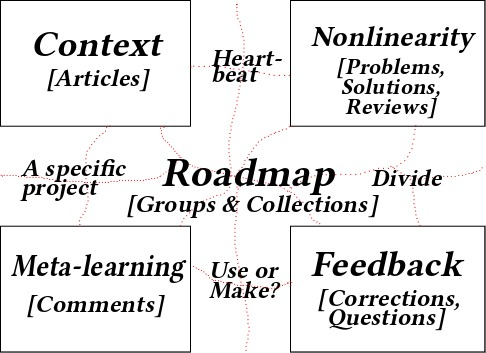
\includegraphics[width=.7\textwidth]{../pictures/PeeragogyEDU-paths.jpg}
\end{center}
\caption*{Peeragogy patterns as loci for ``paths in the grass''}
\end{figure}

\subsection{Initial thematic analysis}

Before describing the new patterns, I will briefly summarize the themes
I identified in the interviews. This can serve as an overview of the
current features and shortcomings of PlanetMath system for people who
are not familiar with it.

\begin{itemize}
\item
  \textbf{``Necessary but not sufficient''.} Users identified a range of
  essential features, like a critical mass of other users to talk to.
\item
  \textbf{``Nice to have''.} It was also easy to identify a bunch of
  cool new ``dream'' features.
\item
  \textbf{Challenges with writing mathematics.} PlanetMath uses LaTeX,
  which isn't entirely easy to learn (however, we could adapt the
  software to help new users get started).
\item
  \textbf{Progressive problem solving.} The new PlanetMath contains
  problems and solutions, but no easy way to talk about conjectures.
  Users would like a better way to share and discuss work-in-progress.
\item
  \textbf{Personal history, social constructivism.} Better features for
  tracking and, where appropriate, sharing, personal history would help
  users make sense of what's happening in the site.
\item
  \textbf{Regulating learning in a social/mediated context.} Different
  users would look for different things to keep them on track (e.g.
  expert guidance, or a due ``sense of urgency'' in feedback from
  peers).
\item
  \textbf{Comparison with roles in other contexts.} Many users expect a
  ``service delivery'' style that is not entirely consistent with the
  ``open'' production model used in a free/open, volunteer-driven
  project. We need to work more on responsiveness in every aspect of the
  project (keeping in mind that most participants are volunteers).
\item
  \textbf{Concreteness as a criterion of quality.} ``Knowing what you
  can do,'' both with the software and with the content, is important.
  On the content level, pictures help.
\item
  \textbf{Personalization and localization.} The system has a
  practically unlimited potential for personalization, although many
  basic personalized interaction modes have not been built yet.
\end{itemize}
\subsection{Pattern analysis}

At the next level of analysis, the themes extracted above were further
analysed in relationship to the peeragogy pattern catalog.

\subsubsection{Frontend and Backend}

Although mathematics is a relatively formal domain, many of the
motivations for using PlanetMath map onto what Zimmerman and Campillo
call informal problem solving {[}3{]}. Informal problems are are
personally defined and possess openended boundary conditions, i.e., are
situated within an ``open world.'' ``Formal'' motivations are are more
likely to be addressed by some variant of a ``look-up'' approach - for
instance, many such problems can be solved by reading the manual. They
do not require the complex, discursive, process of peer supported
problem solving. Acquaintance with the more basic formal features of
mathematical problem solving are typically seen to be a prerequisite for
the more informal activities of mathematics research. This points to the
continued importance of a coherent body of mathematical knowledge in the
form of a well-structured reference resource. This dichotomy suggest a
new and important pattern. This pattern could be called Frontend and
Backend. The ``frontend'' of a system is typically associated with the
formal structural features, while the backend is often associated with
``informal features.'' The Frontend and Backend pattern is related to
the pattern of the ``Newcomer'' pattern, since typically one will not
expect the user of a system to know how to, or to be motivated to, work
with backend features of a system until they have mastered at least some
of the frontend features. It would be rare to find an auto mechanic who
did not know how to drive. David Cavallo wrote about an ``engine
culture'' in rural Thailand, in which structurally open systems made
some of the ``backend'' features of internal combustion engines a part
of daily life {[}4{]}. In PlanetMath, we have an ``open engine'', but
not necessarily an open engine culture (users expect a level of service
provision). The Frontend and Backend pattern clearly lends itself to
standard service provision, but it can also be part of paragogical
activity. For example, sophisticated and committed users of the
PlanetMath website could focus energy on supporting individual
newcomers, by helping them develop a high-quality sub-site on their
topic of interest ({[}RSP8{]}, {[}RSP10{]}). Such effort would
simultaneously inform the development of backend features, and help
raise the profile of the site as a whole. The pattern is in this way
associated with A Specific Project and with the Divide pattern.

\subsubsection{Spanning Set}

You may be able to get what you need without digging - but if you do
need to dig, it would be very good to get some indication about which
direction to dig in. At the content level, this might be achieved by
using high-level ``topic articles'' as a map to the content. But there
is another broader interpretation of this pattern that related to but
distinct from Frontend and Backend - we call this the Spanning Set. In
general, the Spanning Set might be made up of people, or media objects.
In a standard course model, there is one central node, the teacher, who
is responsible for all teaching and course communication. In large
online courses, this model can be is scaled up:

\begin{quote}
\textbf{Anonymous study participant}: {[}E{]}veryone's allocated a
course tutor, who might take on just a half-dozen students - so, they're
not the overall person in charge of the course, by any means.
\end{quote}
Another version is the classical master/apprentice system, in which
every apprentice is supervised by a certified master. In the typical
online Q\&A context, these roles are made distributed, and are better
modeled by power laws than by formal gradations. A ``spanning set'' of
peer tutors could help shift the exponent attached to the power law in
massive courses. We can imagine a given discussion group of 100 persons
that is divided according to the so-called
\href{http://www.wikipatterns.com/display/wikipatterns/90-9-1+Theory}{90/9/1
rule}, so that 90 lurk, 9 contribute a little, and 1 creates the
content. This is what one might observe, for example, in a classroom
with a lecture format. We could potentially shift the system by breaking
the group up, so that each of the 9 contributors leads a small group of
10 persons, at which point, chances are good that some of the former
lurkers would be converted into contributors. At a more semantic level,
we can advance the five paragogical principles and their various
analogues as a candidate description of the fundamental categories and
relationships relevant to peer learning. In practice, principles can
only provide the most visible ``frontend'', and an actual spanning set
is comprised of emergent patterns. In PlanetMath, this would arise from
combining several different features, like a ``start menu'' that shows
what can be done with the site, a Heartbeat built of recurring meetings,
and topic-level guides to content. (Note: as a project with an
encyclopedic component, PlanetMath itself can be used to span and
organize a significantly larger body of existing material.)

\subsubsection{Minimum Viable Project}

The Minimum Viable Product approach to software development is about
putting something out there to see if the customer bites {[}5{]}.
Another approach, related to the pattern we just discussed, is to make
it clear what people can do with what's there and see if they engage. We
might call this the Minimum Viable Project, an adjunct to the
``Roadmap'' pattern, and a new interpretation of the earlier pattern A
Specific Project. One way to strengthen the PlanetMath project as a
whole would be to focus on support for individual projects. The front
page of the website could be redesigned so that the top-level view of
the site is project focused. Thus, instead of collecting all of the
posts from across the site - or even all of the threads from across the
site - the front page could collect succinct summary information on
recently active projects, and list the number of active posts in each,
after the model of Slashdot stories or StackExchange questions. For
instance, each Mathematics Subject Classification could be designated as
a ``sub-project'', but there could be many other cross-cutting or
smaller-scale projects.

\begin{figure}[h]
\begin{center}
\textbf{Frontend and Backend} (\emph{pragma}) \\ Principles and features

\medskip
\textbf{Minimum Viable Project} (\emph{praxis}) \\ A Specific Project,
Roadmap, Heartbeat, Divide, Use or Make

\medskip
\textbf{Spanning Set} (\emph{pratto}) \\ Paths in the grass
\end{center}
\caption*{Paragogical emergent design: a tool for conviviality}
\end{figure}

\subsection{Summary}

This chapter has used the approach suggested by Figure 2 to expand the
peeragogy pattern language. It shows that the peeragogy pattern language
provides a ``meta-model'' that can be used to develop emergent order
relative to given boundary conditions. As new structure forms, this
becomes part of the boundary conditions for future iterations. This
method is a suitable form for a theory of peer learning and peer
production in project-based and cross-project collaborations - a tool
for conviviality in the sense of Ivan Illich. Although this model is
informal, it does suggest one direction for answering the technical
questions posed at the outset of the chapter: in peeragogy, we can
measure learning as a feature of the growth and refinement of the
pattern catalog.


\subsection{References}

\begin{enumerate}
\item
  Gabriel, R. (1996). Patterns of Software. Oxford University Press New
  York.
\item
  Luckin, R. (2010). Re-designing learning contexts: technology-rich,
  learner-centred ecologies. Routledge.
\item
  Zimmerman, B. J. \& Campillo, M. (2003). Motivating self-regulated
  problem solvers. In J. Davidson \& R. Sternberg (Eds.), The psychology
  of problem solving (pp. 233-262). Cambridge University Press New York,
  NY.
\item
  Cavallo, D. P. (2000). Technological Fluency and the Art of Motorcycle
  Maintenance: Emergent design of learning environments (Doctoral
  dissertation, Massachusetts Institute of Technology).
\item
  Ries, E. (2011). The Lean Startup: How today's entrepreneurs use
  continuous innovation to create radically successful businesses. Crown
  Pub.
\end{enumerate}
